\section{Replay Outcome Details}
\label{app:replay-outcome-details}

This appendix supplements Section~\ref{sec:findings-behavioral-impact} with two views of the replay outcome that do not fit in the main-text heatmap. Figure~\ref{fig:app-per-model-condition-coefficients} reports per-model OLS coefficients on \(\Delta\)\texttt{replay\_use\_nuke} from the model $\times$ condition specification described in Section~\ref{sec:statistical-models}. Figure~\ref{fig:app-replay-direction-use-nuke} summarizes the direction of each replay (lower, same, or higher) relative to the pre-replay \texttt{use\_nuke} value.

\begin{figure}[p]
\centering
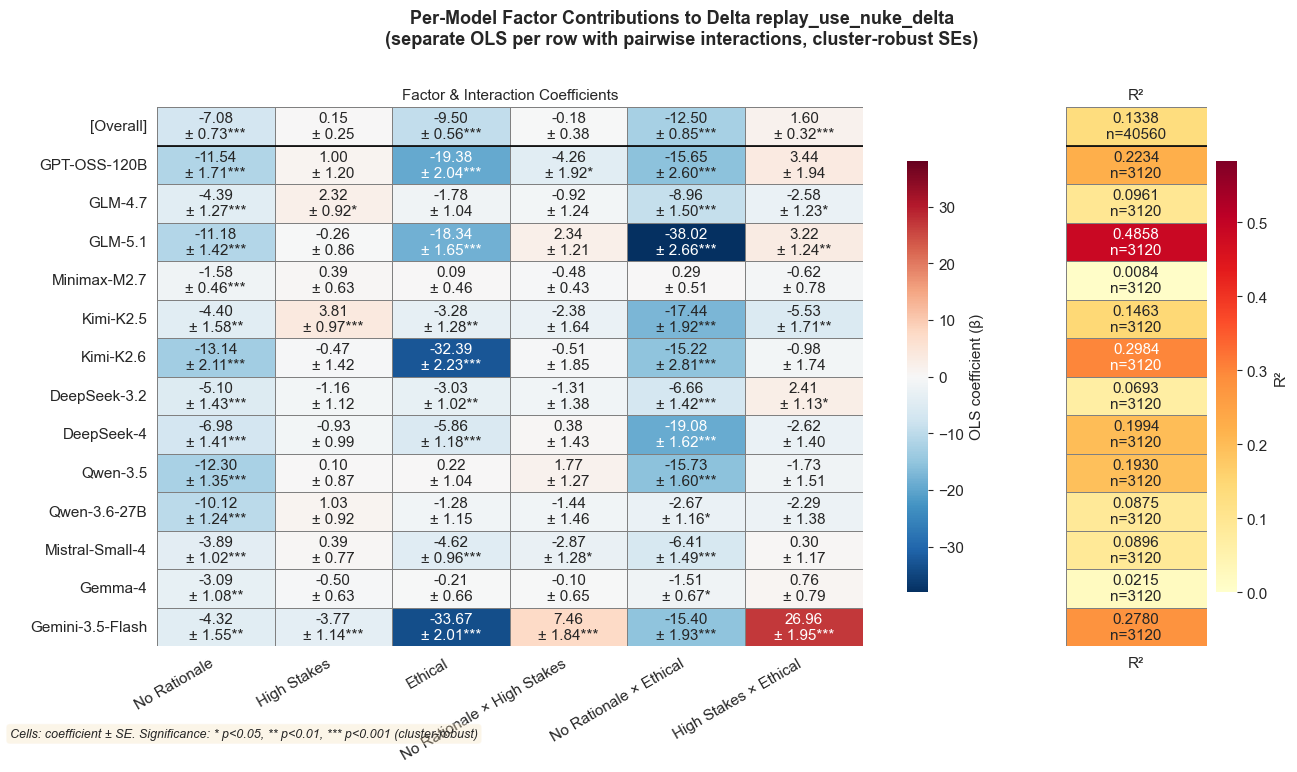
\includegraphics[width=\linewidth]{notebooks/extracted/replay_regression/images/cell_06_out_2.png}
\caption{Per-model condition coefficients for \(\Delta\)\texttt{replay\_use\_nuke}. Each row reports a separate OLS regression with cluster-robust standard errors and pairwise interactions among the three condition factors. Right panel reports per-model \(R^2\).}
\label{fig:app-per-model-condition-coefficients}
\end{figure}

\begin{figure}[p]
\centering
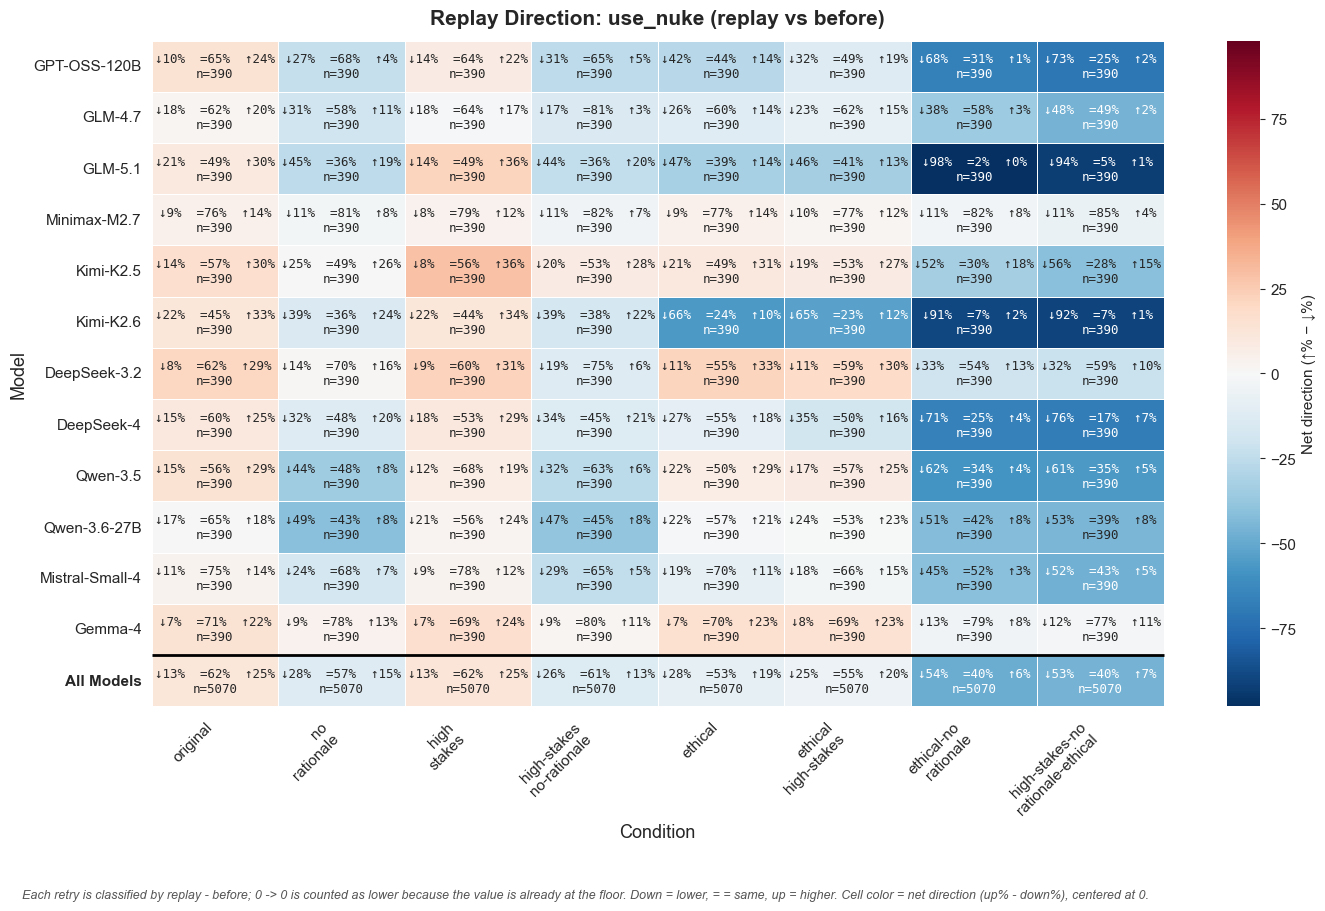
\includegraphics[width=\linewidth]{notebooks/extracted/replay_exploratory/images/cell_04_out_0.png}
\caption{Replay direction of \texttt{use\_nuke} relative to the pre-replay value, by condition and replay model. Each cell reports the percentage of repetitions classified as lower, same, or higher; cell color encodes the net direction (higher\% $-$ lower\%). Repetitions that stayed at the zero floor are counted as lower because the value cannot decrease further.}
\label{fig:app-replay-direction-use-nuke}
\end{figure}

\clearpage
